\documentclass[11pt]{extarticle}
\usepackage{manualdoprofessor}
\usepackage{fichatecnica}
\usepackage{lipsum,media9}
\usepackage[justification=raggedright]{caption}
\usepackage[one]{bncc}
\usepackage[acorde]{../edlab}
\usepackage{marginnote}
\usepackage{pdfpages}
\usepackage[printwatermark]{xwatermark}
%\newwatermark[pagex=2]{
\includegraphics[scale=3.3]{watermarks/test-a.png}}	% página específica
%\newwatermark[oddpages]{
\includegraphics{watermarks/test-a.png}}			% páginas ímpars
%\newwatermark[evenpages]{
\includegraphics{watermarks/test-a.png}}			% págimas pares
%\newwatermark[allpages]{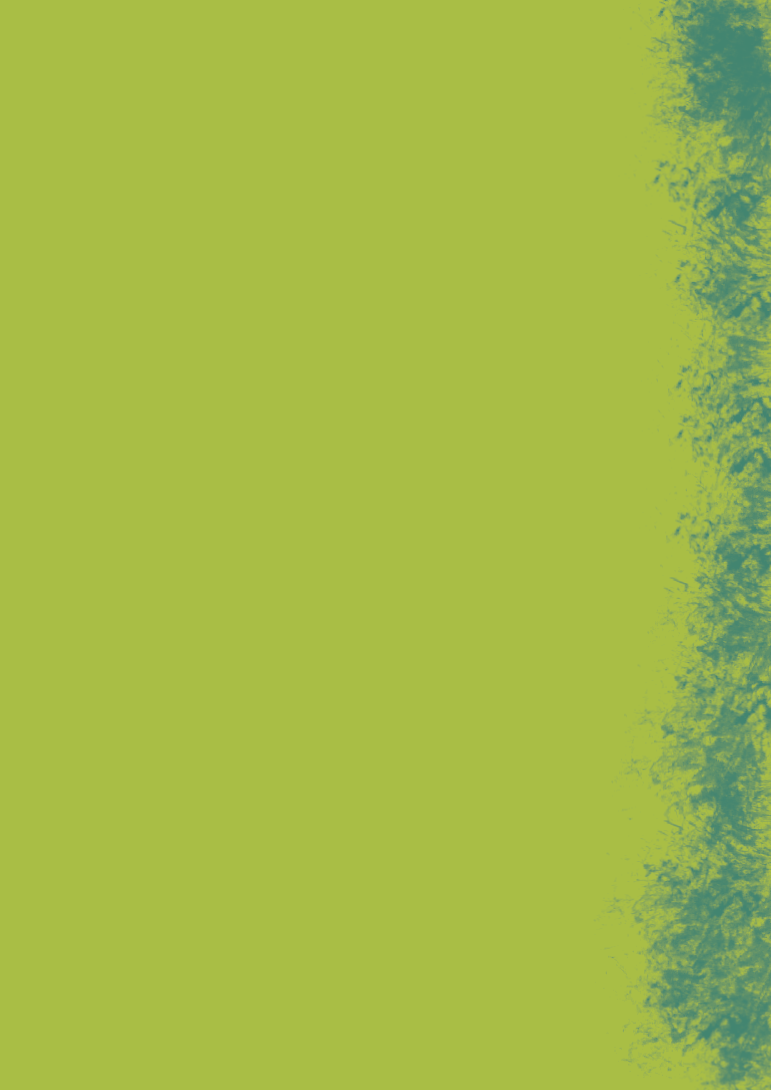
\includegraphics[scale=3.3]{watermarks/test-b.png}}
%\pagecolor{cyan!0!magenta!10!yellow!28!black!28!}

\newcommand{\AutorLivro}{Patience Epps e Danilo Paiva Ramos (Org.)}
\newcommand{\TituloLivro}{Os cantos do homem-sombra}
\newcommand{\Genero}{Lendas, mitos, fábulas}
%\newcommand{\imagemCapa}{./images/PNLD2022-001-01.jpeg}
\newcommand{\issnppub}{978-65-99441-24-0}
\newcommand{\issnepub}{978-65-99441-27-1}
% \newcommand{\fichacatalografica}{PNLD0001-00.png}
\newcommand{\colaborador}{Gabriela Karam}

\begin{document}

\title{\TituloLivro}
\author{\AutorLivro}
\def\authornotes{\colaborador}

\date{}
\maketitle

%\begin{abstract}\addcontentsline{toc}{section}{Carta ao professor}
%\pagebreak

\tableofcontents


\begin{abstract}

Este material tem a intenção de contribuir para que vocês desenvolvam um trabalho aprofundado com a obra \textit{Os cantos do homem-sombra} em sala de aula.
Vocês encontrarão informações sobre o autor, sobre o gênero e também 
algumas propostas de trabalho para a sala de aula que poderão ser exploradas livremente, 
da forma que vocês considerarem mais apropriada para os seus estudantes.

A obra traz um mito indígena passado de geração em geração pela via oral e transcrito por meio da parceria de educadores indígenas com linguistas e antropólogos para criar um modo de escrever a língua e compreender seus princípios gramaticais. Será de grande valia seguirmos juntos na construção de estudantes que estejam inteirados acerca da variedade linguística existente no país, bem como indivíduos que tenham, em sua formação, um contato inicial com os povos que originaram o Brasil.

Com autoria de Patience Epps e Danilo Paiva Ramos, autores que trabalham há anos com o povo indígena Hupd'äh, \textit{Os Cantos do Homem-Sombra} é um livro que traz aos leitores a sensação de fazer parte, de alguma forma, das tantas histórias desse povo que constantemente, ao andar pela mata, depara-se com outros tipos de gente, como a gente-sombra, a gente-onça e a gente-árvore. Aqui você terá informações sobre os escritores da obra, o gênero e os temas trabalhados ao longo dessa história. 

Atualmente os Hupd'äh vivem em aldeias espalhadas pela floresta amazônica, na região do Alto Rio Negro, fronteira entre Brasil e Colômbia. Seu idioma, Hup, é o primeiro a ser ensinado para as crianças, que estão divididas em 35 aldeias, totalizando 1500 pessoas na população total. O português compartilha as páginas com a língua Hup, de modo que os estudantes poderão se familiarizar com essa escrita. Trata-se de uma língua tonal, idioma em que a entonação faz parte da estrutura semântica: uma mesma palavra pode assumir diferentes significados, dependendo do tom de suas sílabas. A obra conduz informações preciosas para aqueles que não têm intimidade com a cultura indígena, trazendo um rico solo para debates e atividades estudantis.

A história é contada com uma atmosfera de lenda: um homem Hup se encanta ao ouvir as canções de um homem-sombra, Way Naku, que está em cima de uma árvore de cucura. Aquele, acostumado a ouvir sobre como estes homens se assemelham a pessoas humanas e carregam em si muita força, sabedoria e poder, mas podem ser perigosos, causar doenças, matar e comer a carne e o espírito dos humanos, sucumbe à beleza sonora e senta ao pé da árvore sem ser visto; começa a pescar num igarapé e segue ouvindo os \textit{caapivaiá} (cantos alegres de festa) proferidos. O homem Hup passa a noite toda e o próximo dia inteiro ouvindo os cantos e acaba registrando em si a cantoria desconhecida. Mas no próximo amanhecer, bate com um machado no tronco da árvore e Way Naku cai e é pego por um jacaré, de modo que o homem pôde fugir e voltar para casa. A narrativa, que traz três estímulos para serem refletidos: a língua portuguesa, a língua Hup e ilustrações repletas de signos, nos encaminha a conhecer a história do primeiro homem que soube cantar os cantos de festas e passou a tradição adiante. 

Promovendo questões como: Onde buscar e conhecer as raízes de nossas tradições em meio a uma globalização que nos confunde a respeito de nossas origens? Como provocar nas crianças a percepção de que os costumes indígenas são parte de nossa cultura? Como aproximar nossa vivência contemporânea à dos Hupd'äh e aprender com esse povo tão antigo e dotado de tanta sabedoria? 

Ao longo do manual, todos esses aspectos serão explorados e relacionados a sugestões de atividades. Com isso, objetiva-se oferecer algumas ideias e inspirações para um trabalho que pode ser desenvolvido tanto a curto, quanto a médio e longo prazo. Sinta-se à vontade para personalizar a aula e torná-la sua, aplicando seus conhecimentos, sua 
personalidade e aproveite para fortalecer seu vínculo com a turma.
Boa aula!

\end{abstract}

\section{Sobre o livro}

A obra se inicia com uma contextualização a respeito dos povos Hupd'äh, contando, na atmosfera de lenda, sobre como esse povo conta muitas histórias sobre pessoas que, andando pela mata, se encontraram com o que chamam de gente-sombra. Esses homens e mulheres-sombra são conhecidos por serem muito fortes e perigosos, além de trazerem muita sabedoria ancestral. Ouve-se dos homens Hup que esses seres podem causar doenças e mesmo comer a carne e o espírito dos humanos. Portanto, deve-se buscar tomar distância deles. Depois de inteirar o leitor, o livro nos leva para um encontro de um homem Hup com um homem-sombra, Way Naku. Diferentemente do que se esperaria, o choque das duas figuras não acontece de maneira afrontosa: o homem Hup se encanta com o canto de Way Naku. Ele se mantém longe da visão deste, mas passa uma noite inteira aprendendo os cantos. No final do dia seguinte, o homem Hup bate com um terçado no tronco de uma árvore de cucura, o homem-sombra acaba sendo pego por um jacaré e nosso Hupd'äh consegue fugir e voltar para casa. O livro nos conta que essa é a história do primeiro homem Hup que soube cantar os cantos das festas - recitadas até hoje pela aldeia. Além de nos trazer a história desse povo, a obra vai além: nos coloca de frente para a língua Hup mostrando, em cada página, a história narrada em português e em Hup. Além disso, ao final do livro, o leitor é inteirado do vocabulário por meio de um rico glossário, bem como um texto sobre os povos Hupd'äh, que traz um mapa para mostrar onde se encontram nos dias de hoje e como vivem e até mesmo uma breve abertura acerca do processo de feitura do livro, permitindo que aqueles que entraram em contato com a obra se sintam parte de tudo isso.

\section{Sobre os autores}

Patience Epps é linguista, professora da Universidade do Textas em Austin e trabalha com os Hupd'äh desde 2000. Danilo Paiva Ramos é antropólogo, doutor em antropologia social pela Universidade de São Paulo e trabalha com os Hupd'äh desde 2006. Anita Ekman é a ilustradora do livro e atualmente mora na Austrália. 

\SideImage{A autora Patience Epps (site: https://thedailytexan.com)}{PNLD2023-017-02.png}
\SideImage{A autora Anita Ekman (site: https://www.goethe.de/ins/br)}{PNLD2023-017-03.png}

\section{Sobre o gênero}

\paragraph{O gênero} O gênero deste livro é \textit{lendas, mitos, fábulas}.

A lenda e o mito são narrativas fantasiosas transmitidas pela tradição oral através dos tempos. De caráter fantástico, as lendas e os mitos combinam fatos reais e históricos com fatos que não têm comprovação de acontecimento, a não ser pela palavra dos que sobraram para contar a história. As lendas e mitos de uma sociedade são fundamentais para que entendamos quem são essas pessoas e no que acreditam, bem como suas tradições. Uma lenda é verdadeira até que se prove o contrário. Com exemplos bem definidos em todos os países do mundo, as lendas e os mitos de um povo geralmente fornecem explicações plausíveis, e até certo ponto aceitáveis, para coisas que não têm explicações científicas comprovadas, como acontecimentos misteriosos ou sobrenaturais.

\Image{A lenda e o mito são narrativas fantasiosas transmitida pela tradição oral através dos tempos (The ponta cabeça; CC-BY-SA-4.0 )} {PNLD2023-017-04.png}

\paragraph{Descrição} A fábula é uma narrativa curta em que os personagens principais geralmente são seres personificados. Esses seres apresentam características humanas, tais como a fala e traços de personalidade. Essas personagens podem ser também objetos animados ou deuses. Em cada história há uma ``lição de moral'': uma mensagem de cunho educativo que busca conscientizar o leitor. A fábula veio do conto, mas se diferencia pela centralidade dos personagens animais e pelo intuito de concluir a história com um ensinamento. É uma história que pode ser contada em prosa ou em versos. 

Sobre a origem da fábula, Douglas Tufano afirma que:

\begin{quote} A fábula teria nascido provavelmente na Ásia Menor e daí teria passado pelas ilhas gregas, chegando ao continente helênico. Há registros sobre fábulas egípcias e hindus, mas sua criação é atribuída à Grécia, pois é onde a fábula passa a ser considerada como um tipo específico de criatividade dentro da teoria literária. 

Na Grécia, os primeiros exemplos de fábula datam do século VIII a.C. Isso nos mostra, é claro, que Esopo não foi o inventor do gênero, mas sim o mais conhecido fabulista na Antiguidade como autor e narrador dessas pequenas histórias.\footnote{\textsc{tufano}, Douglas. Esopo --- Fábulas completas. São Paulo: Moderna, 2015.}
\end{quote}

Esopo foi um autor da Grécia Antiga a quem são atribuídas algumas das mais famosas fábulas, como \textit{A raposa e o cacho de uvas} e \textit{A galinha de ovos de ouro}. Diversas de suas histórias foram recontadas por La Fontaine, que é também um dos mais clássicos fabulistas já existentes.


\section{Proposta de Atividades}
\subsection{Pré Leitura}

A seguir você encontrará a descrição de uma aula modelo como exemplo prático de exploração do livro com estudantes. Esta seção apresentará orientações sobre como organizar a sala de aula para receber os estudantes, exercitar a interação entre eles e prepará-los para que o momento da leitura tenha mais riqueza de conteúdo.

\paragraph{Tema} Povos indígenas do Brasil.  

\paragraph{Conteúdo} Identificação de territórios étnico-culturais brasileiros e reflexão sobre sustentabilidade. 

\paragraph{Objetivo} Apresentar aos estudantes a multiplicidade de territórios étnico-culturais brasileiros e associá-la ao debate a respeito das diferentes formas de relacionar-se com a natureza.  

\paragraph{Justificativa} Muitos alunos desconhecem a riqueza da multiplicidade de territórios étnico-culturais brasileiros e ainda reproduzem estereótipos a respeito das culturas indígenas. A apresentação de \textit{Os Cantos do Homem-Sombra} serve de introdução a essa diversidade, além de servir de ponto de partida para a reflexão a respeito de uma diferença central entre a cultura dominante no Brasil, de matriz europeia e ocidental, e a dos povos originários: a relação com a natureza. Enquanto os primeiros a veem como \textit{recurso}, os indígenas se identificam com ela, veem-se como parte dela.      

\paragraph{Metodologia} Antes de mergulhar na história que esses povos originários nos contam, bem como o glossário, a explicação de quem são os Hupd'äh e o processo de criação do livro, elementos todos presentes na obra, a turma pode entrar em contato com o mapa do Brasil e localizar as diversas aldeias que ainda existem. O professor pode ainda sugerir que usem lápis de cor para diferenciar os povos e seus idiomas. Para isso, incentive e auxilie na pesquisa em livros da biblioteca da escola e em \textit{sites} da internet. Ainda com lápis de cor, escolha uma região e peça para que os estudantes desenhem como eles imaginam essa região. Mostre algumas referências sobre a Amazônia, tribos indígenas e árvores anciãs. Quando os desenhos estiverem prontos e pintados e os estudantes satisfeitos, cole-os nas paredes em volta de toda a sala de aula, com a colaboração de todos. Ainda juntos, construir com papel e cola uma fogueira de papel, criando as madeiras e o fogo, deixando em 3D, colocando-a bem no centro da sala para que se crie a atmosfera da contação de histórias.

\BNCC{EF15AR04}%Experimentar diferentes formas de expressão artística (desenho, pintura, colagem, quadrinhos, dobradura, escultura, modelagem, instalação, vídeo, fotografia etc.), fazendo uso sustentável de materiais, instrumentos, recursos e técnicas convencionais e não convencionais.
\BNCC{EF03GE03}%Reconhecer os diferentes modos de vida de povos e comunidades tradicionais em distintos lugares.
\BNCC{EF04GE06}%Identificar e descrever territórios étnico-culturais existentes no Brasil, tais como terras indígenas e de comunidades remanescentes de quilombos, reconhecendo a legitimidade da demarcação desses territórios.
\BNCC{EF05GE11}%Identificar e descrever problemas ambientais que ocorrem no entorno da escola e da residência (lixões, indústrias  poluentes, destruição do patrimônio histórico etc.), propondo soluções (inclusive tecnológicas) para esses problemas.

\Image{A turma agora pode finalmente se sentar em roda com a floresta em volta. (Suresh K. Nair;CC BY-SA 4.0)}{PNLD2023-017-05.png}

A turma agora pode finalmente se sentar em roda com a floresta em volta e a fogueira no centro. O educador pode partir para o primeiro debate: sobre o trabalho coletivo, a sua eficácia e o prazer da união para construir algo juntos. Logo depois, associar com o trabalho realizado nas aldeias indígenas para construção das ocas, para a alimentação das pessoas e para a melhor convivência entre cada um. E que muito antes dos portugueses chegarem ao Brasil, já se vivia aqui e desse jeito, em conjunto e todos nós temos internamente esse aprendizado. Leia a seguir sobre a habilidade das \textsc{bnccs} abordadas.

Aproveite para estabelecer um paralelo fundamental: esses materiais que foram usados para fazermos nossos desenhos e a fogueira vieram das árvores e podem ter sido ou não reciclados. É interessante trazer à tona a forma como os povos indígenas sempre se conectaram com a natureza - não como um recurso, mas sempre em consonância a ela. Traga para a turma o debate sobre os lixos descartados por nós diariamente e que não reciclamos, seja nas empresas, nas indústrias, em nossas casas e mesmo na escola. É válido questionar de onde vieram esses materiais que foram usados para a atividade e o que se deve fazer com ele após a dinâmica, bem como as possibilidades de reciclagem, reúso e desenvolvimento sustentável. 

\Image{A importância da reciclagem (Grupo Albatroz; Domínio público)}{PNLD2023-017-06.png} 

A \textsc{bncc} define intencionalidade educativa como “organização e proposição, pelo educador, de experiências que permitam às crianças conhecer a si e ao outro e de conhecer e compreender as relações com a natureza, com a cultura e com a produção científica, que se traduzem nas práticas de cuidados pessoais (alimentar-se, vestir-se, higienizar-se), nas brincadeiras, nas experimentações com materiais variados, na aproximação com a literatura e no encontro com as pessoas”.¹ Essa intencionalidade é importante para a condução das atividades propostas no manual, já que situações espontâneas podem surgir a partir dos exercícios e podem se somar às reflexões que a obra e as atividades trazem.

Agora que a turma já se divertiu com o momento artístico, delimitou territórios étnico-culturais brasileiros e refletiu em conjunto sobre as muitas possibilidades de sustentabilidade em comparação à relação com a natureza que os povos originários estabeleceram e seguem até hoje, é hora de aconchegar todos. Reúna as crianças em roda e coloque para tocar \href{https://www.youtube.com/watch?v=7hf4t9u44qs}{as músicas  ``Kêne Kêrane'', de Shaneihu Yawanawa} e \href{https://www.youtube.com/watch?v=IBafJlZxT6s}{``Koangagua'', de Brô MC's}. Dancem em roda de mãos dadas, entusiasme as crianças a tentarem cantar. Após o momento musical, reunidos em roda em volta da fogueira criada e de mãos dadas, explique aos alunos que a arte indígena vive: assim como existem músicas em nossa sociedade, com nossa forma de viver, eles também produzem arte à maneira deles. A partir daí, peça para todos se sentarem na roda e inicie a atividade de leitura. 

\paragraph{Tempo Estimado} Quatro aulas de 50 minutos. 

\Image{``Kanarô'', o povo da queixada na Amazônia (Romerito Aquino; Domínio público)}{PNLD2023-017-07.png} 

¹\textsc{bncc}, página 39

\subsection{Leitura}

\paragraph{Tema} O universo lendário dos povos indígenas.

\paragraph{Conteúdo} A lenda contada em \textit{Os Cantos do Homem-Sombra}.  

\paragraph{Objetivo} Ler e compreender o texto de \textit{Os Cantos do Homem-Sombra} e seus pressupostos culturais. Promover o gosto pelos livros e pela leitura, estimular o desenvolvimento da linguagem, enriquecer o vocabulário e aumentar o conhecimento de mundo.   

\paragraph{Justificativa} O professor tem grande influência na formação de leitores, especialmente quando se trata de compreender e analisar uma lenda indígena, cujo imaginário não faz parte do repertório cultural da maioria dos alunos. É preciso fazer a mediação entre a obra, sua linguagem, suas estruturas, seus pressupostos e os estudantes, de preferência estabelecendo uma relação fundamentada no prazer, na identificação e na liberdade de interpretação. Eis o nosso desafio: ler com os alunos, apresentando as passagens decisivas de um texto, explicando por que elas chamam a atenção e  ouvindo as impressões dos estudantes a respeito de tudo isso.  

\paragraph{Metodologia} A lenda indígena contada na obra traz uma atmosfera interessante para o cenário que foi construído até o momento. As crianças já estão aquecidas com as atividades propostas anteriormente, então é interessante que o clima de história seja mantido. Este é o momento em que será realizada a leitura propriamente dita. Se a escola permitir, é interessante que haja pufes e almofadas para que a turma se sinta em pleno conforto para o momento. É importante que aconteça sem pressa, com a disponibilidade de todos e com prazer. É de grande valia que a leitura seja feita com a participação das crianças. O objetivo da leitura dialogada é que seja uma leitura em bate-papo. A criança deve assumir um papel ativo, mesmo que ainda não seja capaz de ler sozinha. Além de promover o gosto pelos livros, esta prática estimula o desenvolvimento da linguagem, enriquece o vocabulário e aumenta o conhecimento de mundo, além de trazer à criança a sensação de fazer parte da sociedade, uma vez que não se tem a habilidade plena de ler, mas está caminhando nesta direção e seus comentários são levados em conta, provocando possíveis debates e recebendo importância. 

\BNCC{EF35LP03}%Identificar a ideia central do texto, demonstrando compreensão global.
\BNCC{EF35LP05}%Inferir o sentido de palavras ou expressões desconhecidas em textos, com base no contexto da frase ou do texto.
\BNCC{EF35LP12}%Recorrer ao dicionário para esclarecer dúvida sobre a escrita de palavras, especialmente no caso de palavras com relações irregulares fonema-grafema.
\BNCC{EF04LP03}%Localizar palavras no dicionário para esclarecer significados, reconhecendo o significado mais plausível para o contexto que deu origem à consulta.


Recomenda-se que a leitura seja feita com base na identificação das informações básicas da introdução do livro (p.03), que situa os leitores a respeito dos Hupd'äh e suas vivências. Aqui, seguindo a lógica da leitura em bate-papo, é interessante que o professor pergunte como as informações estão chegando para a turma, pedindo que os alunos tragam à tona dúvidas sobre palavras ou expressões desconhecidas e pesquisem nos dicionários da escola esses significados, além de problematizá-los por meio de dúvidas e possíveis debates sobre o tema da palavra - sempre retomando as discussões que aconteceram no momento de pré-leitura para que eles não sejam perdidos. Além disso, o condutor da atividade deve perguntar se o entendimento do texto está acontecendo e retomar a leitura caso haja alguma questão sobre a compreensão da narrativa. É importante que seja explicado à turma que a obra tem mais do que apenas o momento da lenda: há uma contextualização que vem antes e deve ser levada em conta, há um glossário e uma breve explicação a respeito dos povos Hupd'äh - que compõem o grupo de pessoas das quais se falou há pouco: os povos originários. A relação do povo retratado na lenda com a atividade anterior é fundamental.

\subsubsection{Explorando e analisando um dos cantos do Homem-Sombra}


Agora, aproveitando o contexto do livro, que é finalizado com uma das canções do Homem-Sombra, trabalhar com os estudantes as possibilidades de percussão corporal. Para dar início a esse trabalho, é de grande valia que o educador coloque um vídeo com a música \href{https://www.youtube.com/watch?v=_Tz7KROhuAw}{``Samba Lelê'', dos Barbatuques}. Assim, finalizado o vídeo, pode-se orientar que algumas das crianças estejam na voz, outras, nas palmas e outras, na percussão com os pés. A ideia aqui é se apropriar da canção do Homem-Sombra que encerra o livro e mostrar para as crianças que a criatividade é prioridade: a melodia pode ser feita à nossa maneira, bem como a percussão de um texto. 

\Image{A turma reunida em grupo (Paraíba Governo do Estado; Domínio público)}{PNLD2023-017-08.png}


\BNCC{EF15AR13}%Identificar e apreciar criticamente diversas formas e gêneros de expressão musical, reconhecendo e analisando os usos e as funções da música em diversos contextos de circulação, em especial, aqueles da vida cotidiana.}
\BNCC{EF15AR15}%Explorar fontes sonoras diversas, como as existentes no próprio corpo (palmas, voz, percussão corporal), na natureza e em objetos cotidianos, reconhecendo os elementos constitutivos da música e as características de instrumentos musicais variados.
\BNCC{EF05LP05}%Identificar a expressão de presente, passado e futuro em tempos verbais do modo indicativo.

É interessante que a turma compreenda que o processo de percussão corporal pode ser realizado nos mais diversos textos e poesias as quais entrarem em contato na vida. A atividade demonstra, na prática, que as pessoas podem fazer arte em quaisquer condições e que nosso corpo é um templo que dá possibilidades para que a arte seja feita, assim como os povos indígenas fazem: a partir de suas referências e repertório de vida, realizam arte à sua maneira e com as condições que têm. Este é um bom momento para colocar em questão uma análise da música: 

\textit{Outro galho de cucura
Outro galho de cucura
Eu jogo para baixo
Outro galho de cucura
Eu jogo para baixo
Colho o cacho de cucura
Eu jogo para baixo
Way Naku, yari nóóy mah
Marika, Way Naku}

Nas frases, é possível identificar o uso do tempo presente do modo indicativo. É interessante pedir aos alunos que façam essa análise, identificando o tempo e modo verbal da música e qual o sentido das frases, o que a música quer dizer e os motivos pelos quais houve a escolha verbal da música. A partir daí, é possível passar um exercício em que os alunos passem o texto para os passados e presentes do indicativo (pretérito perfeito, pretérito imperfeito, pretérito mais-que-perfeito, futuro do presente e futuro do pretérito), analisando a diferença de sentido que a mudança provoca. 

\paragraph{Tempo Estimado} Duas aulas de 50 minutos. 

\subsection{Pós-leitura}

\paragraph{Tema} Oralidade e escrita.

\paragraph{Conteúdo} Preservação de tradições coletivas por meio da oralidade e da escrita: limites e alcances. 

\paragraph{Objetivo} Promover entre os alunos a percepção da importância da ancestralidade e da preservação de sua cultura por meio da oralidade e da escrita.  

\paragraph{Justificativa} Histórias familiares são integrantes fundamentais do repertório de nossos estudantes. Distinguir registros orais e escritos desse cabedal afetivo é uma forma de respeitar diferenças linguísticas e permitir a percepção de que há variantes adequadas a contextos distintos, que também será exercitada por meio da encenação da lenda.      

\paragraph{Metodologia}

Após a leitura, pode-se iniciar um momento reflexivo. Neste momento, o educador dá início à próxima parte da atividade. Incentive os estudantes a contarem histórias ou lendas que já ouviram de seus pais ou avós e assim, abrir o debate acerca da importância da tradição oral. É interessante que o educador peça que os estudantes se preocupem com a concordância dos verbos e pronomes para darem seus depoimentos e contarem suas histórias. Veja as \textsc{bnccs} que se relacionam à atividade: 

\Image{Incentive os estudantes a contarem histórias ou lendas que já ouviram de seus pais ou avós (Município de Modelo; Domínio público)}{PNLD2023-017-09.png}

\BNCC{EF05LP06}%Flexionar,adequadamente, na escrita e na oralidade, os verbos em concordância com pronomes pessoais/nomes sujeitos da oração.
\BNCC{EF04LP05}%Identificar a função na leitura e usar, adequadamente, na escrita ponto final, de interrogação, de exclamação, dois-pontos e travessão em diálogos (discurso direto), vírgula em enumerações e em separação de vocativo e de aposto.
\BNCC{EF01HI01}%Identificar aspectos do seu crescimento por meio do registro das lembranças particulares ou de lembranças dos membros de sua família e/ou de sua comunidade.

Depois que todos contarem suas histórias e comentarem acerca do que foi dito, peça para que eles redijam a história de que mais gostaram, preocupando-se em escrever uma história na mesma atmosfera mitológica que a obra e também com as concordâncias verbais com pronomes pessoais/nomes e sujeitos da oração. Peça para que cada um leia o que foi escrito e analise morfologicamente cada expressão usada em seus textos. Além disso, peça para que utilizem o discurso direto para que experimentem o uso de travessões, bem como vírgulas usadas corretamente e o uso de vocativo e aposto quando necessário. Corrija-os em caso de erros e aproveite o momento para revisar a matéria se houver dificuldades.

\subsubsection{A leitura e a escrita: um encontro valioso}

Se na pré-leitura mergulhamos na história dos povos originários e em como eles estão vivendo atualmente, agora é o momento de entendermos a importância da vida deles para a nossa forma de viver. Peça para que os alunos se organizem em pequenos grupos e contem, de forma criativa, utilizando-se de recursos teatrais, a história que foi ouvida dos Hupd'äh. Oriente-os a utilizarem inclusive o conteúdo do livro que traz informações sobre esse povo e onde vivem.

\BNCC{EF15AR20}%Experimentar o trabalho colaborativo, coletivo e autoral em improvisações teatrais e processos narrativos criativos em teatro, explorando desde a teatralidade dos gestos e das ações do cotidiano até elementos de diferentes matrizes estéticas e culturais.


De forma organizada, enumere os grupos e comece o espetáculo. Depois que todas as crianças se apresentarem, peça que todos retornem à roda e comentem sobre os exercícios dos colegas, incitando-os a trazerem informações como o uso verbal dos colegas e os efeitos que esses usos geraram dramaticamente. 

\Image{De forma organizada, enumere os grupos e comece o espetáculo (Município de Modelo; Domínio público)}{PNLD2023-017-10.png}


\subsubsection{Refletindo sobre as atividades}

\BNCC{EF15AR25}%Conhecer e valorizar o patrimônio cultural, material e imaterial, de culturas diversas, em especial a brasileira, incluindo-se suas matrizes indígenas, africanas e europeias, de diferentes épocas, favorecendo a construção de vocabulário e repertório relativos às diferentes linguagens artísticas.

É importante que os alunos estejam familiarizados com os motivos que levaram o educador a proporcionar as atividades do dia e mesmo questioná-los sobre a importância de entrar em contato com a necessidade de conhecermos a cultura indígena, de modo que conhecer esses povos nos faz conhecer a nós mesmos. Além disso, é interessante que o professor se preocupe em trazer aos alunos a ótica de que compreender verbos e seus usos é fundamental para que eles possam se organizar mentalmente, bem como se comunicar no mundo. O contato com a arte indígena deve ser levado em conta também, na medida em que os estudantes se divertiram com as músicas e perceberam que a arte não está restrita apenas à estrutura ocidental europeia, há diversas fontes artísticas que podem ser contempladas e mesmo feitas por nós, principalmente para que entendamos a diversidade existente no mundo, e mesmo em nosso país.

\paragraph{Tempo Estimado} Duas aulas de 50 minutos. 

\section{Sugestões de referências complementares}

\subsection{Livros} 

\begin{itemize}
\item \textsc{krenak}, Ailton. \textit{Ideias para adiar o fim do mundo}. São Paulo: Companhia das Letras, 2019.

Livro sobre crítica da ideia de humanidade como algo separado da natureza, de uma ``humanidade que não reconhece que aquele rio que está em coma é também o nosso avô''.

\item \textsc{munduruku}, Daniel. \textit{Contos indígenas brasileiros}. São Paulo: Global Editora, 2004.

Livro que traz contos dos povos originários e apresenta a diversidade cultural e linguística no Brasil.
\end{itemize}

\subsection{Artigos}

\begin{itemize}
\item \textsc{alves}, Francielle Thalita Almeida, \textsc{prates}, Elton Junio Sady, \textsc{carneiro} Luis Henrique Prado, \textsc{de sá}, Ana Carolina Micheletti Gomide Nogueira, \textsc{pena}, Érica Dumont e \textsc{malta}, Deborah Carvalho. Mortalidade proporcional nos povos indígenas no Brasil nos anos 2000, 2010 e 2018. 
In: \href{https://www.scielo.br/j/sdeb/a/DjX5mjjj5GjMVrHnMsnvKVx/?format=pdf&lang=pt}{Saúde Debate. V.45, p. 691-706, jul-set 2021}. 
Acesso em 13 dez 2021. 

Artigo acadêmico que discorre sobre os índices de mortalidade nos povos indígenas em 2000, 2010 e 2018. 

\item \textsc{coelho}, Tayane da Rocha Costa, \textsc{sampaio}, Henrique Bonione Carneiro, \textsc{araujo}, Nara Santos e \textsc{cury}, Patricia Ramos. \href{https://www.scielo.br/j/csc/a/5dWp6FdB4zs6Y8cZtjDXQqD/?lang=pt}{Indicação de exodontias e fatores associados: estudo transversal na população indígena Kiriri}.  

Artigo acadêmico que traz uma etnografia detalhada dos povos Kiriri.  
\end{itemize}

\section{Bibliografia comentada}
\subsection{Livros}

\begin{itemize}
\item \textsc{brasil}. Ministério da Educação. Base Nacional Comum Curricular. Brasília, 2018.

Consultar a \textsc{bncc} é essencial para criar atividades para a turma. Além de especificar quais habilidades precisam ser desenvolvidas em cada ano, é fonte de informações sobre o processo de aprendizagem infantil. 

\item \textsc{seabra}, Carlos. O livro dos jogos das crianças indígenas e africanas. São Paulo: Estrela, 2019.

Nesse livro, o leitor vai conhecer a origem e a prática de jogos que resgatam a riqueza das culturas indígenas e africanas, matrizes fundamentais do que constitui o Brasil. Os povos indígenas brasileiros possuem várias brincadeiras, mas o único “jogo de tabuleiro” conhecido é o adugo ou jogo da onça, que apresentamos aqui para o leitor. Já os povos africanos possuem jogos com centenas e até milhares de anos, sendo os mais conhecidos os mancalas, chamados de “xadrez africano”, dos quais escolhemos 4 variedades. Todos esses jogos permitem exercer o raciocínio lógico e estratégico, além de serem bem divertidos e resgatarem nossas raízes.
 
\item \textsc{wapichana}, Kamuu Dan. Sopro da vida – Putakaryy Kakykary. São Paulo: Expressão Popular, 2019.

De forma simples e didática, o livro caminha entre a luta pela preservação do cerrado brasileiro e a importância de salvaguardar nossas riquezas naturais. Inspirado na história do Santuário dos Pajés, em Brasília, território indígena onde vive o autor, a obra também fala sutilmente sobre a intensa especulação agrária por parte dos ruralistas.

\item \textsc{kopenawa}, Davi e \textsc{albert}, Bruce. A queda do céu - Palavras de um xamã yanomami. São Paulo: Companhia das Letras, 2015.

Um grande xamã e porta-voz dos Yanomami oferece neste livro um relato excepcional, ao mesmo tempo testemunho autobiográfico, manifesto xamânico e libelo contra a destruição da floresta Amazônica. Interessante para trazer mais da realidade brutal na qual se encontram os povos indígenas, que lutam todos os dias por sua sobrevivência. 
\end{itemize}

\subsection{\textit{Sites}}

\begin{itemize}
\item Documentário \href{https://www.youtube.com/watch?v=repPmoz8ozQ}{“Falas da Terra”}.

No documentário, está presente a pluralidade de falas dos diferentes indígenas do Brasil, que compartilham suas identidades étnico-raciais, culturas, lutas e ocupações, tratando não apenas da terra física mas de sua extensão cultural, como moda, música e arte.

\item Página da \textsc{ong} Instituto Socioambiental, com vídeos sobre a situação dos povos indígenas, mostrando formas para defender os povos originários, comunidades tradicionais, direitos humanos e o patrimônio cultural para valorizar a diversidade socioambiental. 

\item Vídeo \href{https://www.youtube.com/watch?v=-aXBbySnijg}{“Povo Karipuna resiste à destruição de suas florestas”} do canal \textit{Greenpeace}. 

Breve vídeo que mostra como o povo Karipuna se organiza para resistir à destruição da floresta onde habitam. Se você achar conveniente, esse vídeo pode ser recomendado para inspirá-los a entender como resistir diante do quadro de desmatamento no Brasil. 
\end{itemize}

\subsection{Filmes}

\begin{itemize}
\item \textit{A Febre}. Dirigido por Maya Da-Rin, 2019.

A Febre é um filme franco-teuto-brasileiro de drama e suspense dirigido por Maya Da-Rin. Falado em português e nas línguas indígenas tukano e tikuna, é escrito por Maya Da-Rin, Miguel Seabra Lopes e Pedro Cesarino, e protagonizado por Regis Myrupu e Rosa Peixoto. Seu elenco principal é composto por atores indígenas do Alto Rio Negro, pertencentes aos Desanos, Tucanos e Tarianas, tendo sido para muitos deles a primeira experiência no cinema.

\item \textit{As hiper mulheres}. Dirigido por Carlos Fausto, Takumã Kuikuro e Leonardo Sette, 2012. 

O filme conta a história de um homem que, temendo a morte de sua esposa idosa, pede a seu sobrinho que realize Jamurikumalu, o ritual feminino máximo do Alto Xingu para que ela possa cantar pela última vez. As mulheres do grupo começam os testes enquanto a única cantora que realmente conhece todas as canções está gravemente doente.

\item \textit{Guerras do Brasil}. Dirigido por Luiz Bolognesi, 2019.

Guerras do Brasil apresenta os fatos e as diferentes narrativas dos principais conflitos armados da História do país. A narrativa é contada por meio de depoimentos dos principais conhecedores dos fatos (historiadores, cientistas sociais, jornalistas). Recomenda-se que seja mostrado o primeiro episódio, que fala a respeito dos conflitos que os povos indígenas enfrentam para sobreviverem em meio à dizimação de seu povo e de suas terras.

\end{itemize}
\end{document} 